\chapter{Το πακέτο Shockwave.jl}
\label{chapter:shockwave}

\section{Σκοπός του πακέτου}

Όπως είδαμε στο κεφάλαιο \ref{chapter:julia-diffeq}, η Julia παρέχει ένα αρκετά ανεπτυγμένο σύστημα επίλυσης συστημάτων συνηθών διαφορικών εξισώσεων (ODE).
Επίσης, στο κεφάλαιο \ref{chapter:theory}, είδαμε πως μπορούμε να επιλύσουμε αριθμητικά το σύστημα μερικών διαφορικών εξισώσεων (PDE) του Euler για την συμπιεστή ροή των ρευστών, κατασκευάζοντας ένα σύστημα συνηθών διαφορικών εξισώσεων που μοντελοποιούν την εξέλιξη των αριθμητικών συντελεστών που ορίζουν την προσέγγιση της λύσης σε κάθε χρονική στιγμή.

Ερχόμαστε λοιπόν στην κύρια συνεισφορά αυτής της εργασίας, η οποία είναι η ανάπτυξη ενός πακέτου το οποίο επιτρέπει την περιγραφή ενός προβλήματος νόμου διατήρησης (conservation law), από την οποία κατασκευάζει ένα σύστημα ODE το οποίο ο χρήστης μπορεί να επιλύσει με την ευελιξία του \jlinl{DifferentialEquations.jl} όπως περιγράφεται στο κεφάλαιο \ref{chapter:julia-diffeq}.
Με αυτόν τον τρόπο, έχουμε μία αναχώρηση από το τυπικό μοντέλο επιλυτών ρευστομηχανικής που συνήθως αποτελούν μεγάλα μονολιθικά προγράμματα.
Με το πακέτο της εργασίας, η μέθοδος πεπερασμένων όγκων και το φυσικό μοντέλο του ρευστού είναι πλέον ένα σύνολο συναρτήσεων και δομών δεδομένων, σχεδιασμένων να μπορούν να ενσωματωθούν σε μεγαλύτερα προγράμματα, ακολουθώντας έτσι την φιλοσοφία σχεδίασης της Julia.
Ως όνομα για το πακέτο επιλέχθηκε ο τίτλος \jlinl{Shockwave.jl}, καθώς ως βασικός στόχος, τουλάχιστον της αρχικής ανάπτυξης, είναι η επίλυση των συμπιεστών εξισώσεων Euler.

Όσον αφορά τον τρόπο περιγραφής του προβλήματος προς επίλυση υπάρχει ένα φάσμα προσεγγίσεων, όπου χρειάζεται να διαλέξουμε ανάμεσα στην συντομία της περιγραφής και στην γενικότητά της.
Στην συγκεκριμένη περίπτωση, αντλούμε έμπνευση από το πακέτο \jlinl{OrdinaryDiffEq.jl} που επιτρέπει την επίλυση συστημάτων ODE, παρέχοντας μία συνάρτηση που υπολογίζει την χρονική παράγωγο σε κάθε χρονική στιγμή, το χρονικό διάστημα ολοκλήρωσης, και τον αλγόριθμο ολοκλήρωσης.
Αντίστοιχα, το πακέτο \jlinl{Shockwave.jl}, περιγράφει ένα πρόβλημα νόμου διατήρησης (conservation law), ή εναλλακτικά μεταφοράς (advection), ως συνδιασμό τριών στοιχείων:

\begin{itemize}
    \item την συνάρτηση υπολογισμού της ροής $\mathbf{F}$ ανάμεσα σε δύο γειτονικά στοιχεία,
    \item το πλέγμα πάνω στο οποίο το πρόβλημα επιλύεται, και
    \item την αριθμητική μέθοδο χωρικής διακριτοποιήσης (π.χ. πεπερασμένοι όγκοι N-τάξης, ασυνεχής μέθοδος Galerkin (Discontinuous Galerkin/DG), κ.α.). Προς το παρόν η μόνη διαθέσιμη μέθοδος είναι οι πεπερασμένοι όγκοι πρώτης τάξης.
\end{itemize}

Έτσι με βάση τα παραπάνω, μπορούμε να ορίσουμε τον τύπο δεδομένων που αναπαριστά ένα τέτοιο πρόβλημα:

{\large
\begin{jllisting}[language=julia,style=jlcodestyle]
struct AdvectionProblem{N, F, D, M}
    # Field names
    fields::NTuple{N, Symbol}

    # Flux function
    f::F

    # Mesh
    m::M

    function AdvectionProblem(fields::NTuple{N, Symbol}, f::F, ::D, m::M) where
            {N, F, D <: AbstractDiscretization, M <: AbstractMesh}
        new{N, F, D, M}(fields, f, m)
    end
end

# Supported discretization methods
struct FV1 <: AbstractDiscretization end # Finite Volume Method - 1st-order
\end{jllisting}
}

Αρχικά παρατηρούμε ότι οι παραμέτροι που αναφέραμε παραπάνω, δεν αποθηκεύονται ως τιμές αλλά ως τύποι δεδομένων.
Αυτό είναι μία συνηθισμένη τεχνική στην Julia καθώς επιτρέπει να ξεχωρίσουμε την λογική που πρέπει να εκτελεστεί κατά την μεταγλώττιση, από αυτήν του χρόνου εκτέλεσης, και μας επιτρέπει να εκφράσουμε τον πολυμορφισμό που θέλουμε χρησιμοποιώντας το σύστημα multiple dispatch.

Επίσης, χρειάζεται να ορίσουμε τα βαθμωτά πεδία του προβλήματος.
Αυτό επιτρέπει να ορίσουμε βοηθητικές συναρτήσεις που αυτόματα εκχωρούν μνήμη για τα δεδομένα της λύσης, και γράφουν τα αποτελέσματα σε αρχεία VTK με κατάλληλες ετικέτες.
Πέρα από αυτό, οι ετικέτες δεν χρειάζονται σε κάτι κατά την διάρκεια της επίλυσης.
Βασικότερος είναι ο ακέραιος \jlinl{N}, που ορίζει τον αριθμό των βαθμωτών πεδίων.

Είπαμε όμως ότι χρειάζεται εν τέλει να παράξουμε μία συνάρτηση η οποία υπολογίζει την χρονική παράγωγο.
Ένας τρόπος να το κάνουμε αυτό, θα ήταν η δυναμική παραγωγή κώδικα και χρήση των λεγόμενων \emph{generated functions}.
Υπάρχει ένας όμως σημαντικά απλούστερος τρόπος να πετύχουμε κάτι παρόμοιο, καθώς η Julia μας επιτρέπει να ορίσουμε μία συνάρτηση για κάθε τύπο δεδομένων, η οποία καλείται εάν καλέσουμε το αντικείμενο σαν συνάρτηση.
Πρακτικά, για τον παραπάνω τύπο \jlinl{AdvectionProblem}, μπορούμε να ορίσουμε μία συνάρτηση της μορφής:

{\large
\begin{jllisting}[language=julia,style=jlcodestyle]
function (p::AdvectionProblem)(du, u, param, time)
    # Compute and fill du
end
\end{jllisting}
}

Με αυτόν τον τρόπο, μπορούμε να χρησιμοποιήσουμε ένα αντικείμενο τύπου \jlinl{AdvectionProblem} ως την συνάρτηση της χρονικής παραγώγου που χρειαζόμαστε για να ορίσουμε ένα \jlinl{ODEProblem}.

\section{Συνάρτηση υπολογισμού ροής}

Η συνάρτηση υπολογισμού της ροής είναι ο μοναδικός τρόπος με τον οποίο ο χρήστης μπορεί να καθορίσει τον φυσικό νόμο του προβλήματος.
Αυτή έχει την μορφή

{\large
\begin{jllisting}[language=julia,style=jlcodestyle]
function F(UL, UR, n)
    SVector(...)
end
\end{jllisting}
}

όπου \jlinl{UL}, είναι ένα διάνυσμα μήκους \jlinl{N}, που περιέχει τους συντελεστές της λύσης στο εσωτερικό του στοιχείου, \jlinl{UR} το διάνυσμα της λύσης στο εξωτερικό του στοιχείου, και \jlinl{n}, το μοναδιαίο διάνυσμα κάθετο στην επιφάνεια του ορίου.
Η συνάρτηση αυτή επιστρέφει ένα διάνυσμα μήκους \jlinl{N} που περιέχει την ροή προς το εξωτερικό του πεπερασμένου όγκου για το κάθε βαθμωτό πεδίο.

\section{Πλέγμα}

Το πλέγμα ορίζει τόσο την τοπολογία των στοιχείων, όσο και την ακριβή γεωμετρία τους στον χώρο.
Ο μοναδικός τύπος πλέγματος που υποστηρίζεται από το πακέτο είναι το δυδιάστατο μη-δομημένο πλέγμα (2D unstructured grid), που αποτελείται από τριγωνικά στοιχεία, αλλά δεν υπάρχει κάτι στην σχεδίαση του πακέτου που να εμποδίζει την μελλοντική προσθήκη, π.χ. δομημένων καμπυλόγραμμων πλεγμάτων (structured curvilinear grid).

Το μη δομημένο πλέγμα, ορίζεται από την δομή δεδομένων \jlinl{UnstructuredMesh}, ως εξής:

{\large
\begin{jllisting}[language=julia,style=jlcodestyle]
@enum ElementType begin
    TriangleElement
    LineElement
end

struct Triangle{F, I}
    vert::SVector{3, I} # Vertices
    n::SVector{3, Vector2{F}} # Normal vectors
    l::SVector{3, F} # Edge lengths
    nb::SVector{3, I} # Neigbors
    area::F # Area
end

struct Line{F, I}
    vert::SVector{2, I}
    l::F # Length
    n::Vector2{F} # Normal vector pointing *into* the domain
    nb::I # Neighbor
end

struct Element{I}
    type::ElementType
    idx::I # Local index
end

struct UnstructuredMesh{AV, AE, AT, AL, F, I} <: AbstractMesh
    # Nodes (vector of Vector2)
    nodes::AV

    # Elements (vector of Element)
    elements::AE

    # Triangles (vector of Triangle)
    triangles::AT

    # Lines (vector of Line)
    lines::AL

    # Marked boundaries
    groups::Array{Int, 2} # (group number, first line index|group size)

    # Group name -> index of group in the groups array
    groupnames::Dict{String, Int}
end
\end{jllisting}
}

Η επιλογή του συγκεκριμένου τρόπου αναπαράστασης του διδιάστατου πλέγματος, έγινε με το σκεπτικό οι προσπελάσεις μνήμης που απαιτούνται σε κάθε επανάληψη να ελαχιστοποιηθούν.
Έτσι, κατά την προεπεξεργασία του πλέγματος, υπολογίζουμε πλήρως όλα τα κάθετα διανύσματα, τα μήκη πλευρών και της επιφάνειες των στοιχείων.
Επίσης, ξεχωρίζουμε τα στοιχεία ανάμεσα σε τρίγωνα και ευθύγραμμα τμήματα, τα οποία αποτελούν τα όρια του υπολογιστικού χώρου.
Το κάθε στοιχείο έχει μία καθολική θέση (global index), και μία τοπική θέση (local index).
Αυτές αναφέρονται στην θέση του στοιχείου στον πίνακα με όλα τα στοιχεία, που έχει ίδια μορφή με το διάνυσμα της λύσης, και στους πίνακες για την κάθε κατηγορία στοιχείου, που περιέχουν τις γεωμετρικές πληροφορίες.
Καθώς τα τρίγωνα είναι σημαντικά περισσότερα και χρειάζεται να τα προσπελάσουμε πολύ περισσότερες φορές, η τοπική και η καθολική τους θέση ταυτίζονται, ενώ για τα ευθύγραμμα τμήματα, διαφέρουν κατά τον αριθμό των τριγώνων, δηλαδή βρίσκονται μετά από όλα τα τρίγωνα στον πίνακα των στοιχείων.

Τα όρια αποτελούνται αποκλειστικά από ευθύγραμμα τμήματα, και στα περισσότερα προγράμματα παραγωγής πλεγμάτων, ο χρήστης μπορεί να τους δώσει μία φιλική ονομασία.
Καθώς τα ευθύγραμμα τμήματα για κάθε όριο είναι αποθηκευμένα στην σειρά, μπορούμε να ορίσουμε ένα όριο με το δίαστημα των θέσεων των ευθυγράμμων τμημάτων από τα οποία αποτελείται, δηλαδή την θέση του πρώτου και του τελευταίο ευθύγραμμου τμήματός του.
Για λόγους απόδοσης, αυτοί οι αριθμοί αποθηκεύονται σε μία συνεκτική (compact) δομή δεδομένων, στην συγκεκριμένη περίπτωση έναν διδιάστατο πίνακα, αλλά οι φιλικές ονομασίες των ορίων είναι διαθέσιμες από το λεξικό \jlinl{groupnames}, και χρησιμοποιούνται κατά τον ορισμό οριακών συνθηκών, όπως θα δούμε στην ενότητα \ref{section:shockwave-bcs}.

Το πακέτο παρέχει την δυνατότητα ανάγνωσης διδιάστατων πλεγμάτων με τριγωνικά στοιχεία στην μορφή που δέχεται ο επιλυτής SU2 \cite{Palacios2013}.
Αυτή η μορφή υποστηρίζεται ως μορφή εξόδου από διάφορα προγράμματα παραγωγής πλεγμάτων, συμπεριλαμβανομένου του λογισμικού ανοικτού κώδικα Gmsh \cite{Gmsh2009}.

\section{Παράδειγμα: μεταφορά βαθμωτού πεδίου σε σταθερό πεδίο ροής}
\label{section:square-advection}

Ως επίδειξη του τρόπου λειτουργίας των τμήματων που περιγράψαμε παραπάνω, ας εξετάσουμε την επίλυση του εξής απλού προβλήματος.
Έστω ότι έχουμε ένα τετράγωνο χώρο, που εκτείνεται από το σημείο $\left(0, 0\right)$ μέχρι το σημείο $\left(1, 1\right)$.
Σε αυτόν τον χώρο, ορίζουμε το εξής διανυσματικό πεδίο ταχύτητας:

\begin{equation*}
    \mathbf{V} = - \sin \pi x \cos \pi y \mathbf{i} + \cos \pi x \sin \pi y \mathbf{j}
\end{equation*}

% todo generate quiver plot of the field

Έστω τώρα ότι σε αυτόν τον χώρο ορίζουμε ένα βαθμωτό πεδίο $U$, του οποίου την μεταφορά θέλουμε να προσομοιώσουμε.
Με άλλα λόγια, θέλουμε να λύσουμε την διαφορική εξίσωση:

\begin{equation*}
    \frac{\mathrm{D} U}{\mathrm{D} t} = \frac{\partial U}{\partial t} + \mathbf{V} \cdot \nabla U =
        \frac{\partial U}{\partial t} + \nabla \cdot \left( \mathbf{V} U \right) = 0
\end{equation*}

όπου $\nabla \cdot \left( \mathbf{V} U \right) = \mathbf{V} \cdot \nabla U$, καθώς $\nabla \cdot \mathbf{V} = 0$.

Συγκρίνοντας την παραπάνω εξίσωση με την \ref{eq:advection-point-form}, προκύπτει η συνάρτηση ροής ως:

\begin{equation*}
    \mathbf{F} = \mathbf{V} U
\end{equation*}

Για να βρούμε την μορφή της συνάρτησης ροής που μπορούμε να χρησιμοποιήσουμε πάνω στο ασυνεχές όριο, ας θεωρήσουμε ότι λύνουμε το πρόβλημα κατά μήκος του κάθετου διανύσματος $\mathbf{\hat{n}}$, παράλληλα στο οποίο ορίζουμε έναν χωρικό άξονα συντεταγμένων, έστω $z$.
Τότε, γραμμικοποιώντας το πρόβλημα, έχουμε:

\begin{equation*}
    \frac{\partial U}{\partial t} + \frac{\partial (\mathbf{V} \cdot \mathbf{\hat{n}}) U}{\partial z} 
    \approx \frac{\partial U}{\partial t} + \left( \mathbf{V} \cdot \mathbf{\hat{n}} \right) \frac{\partial U}{\partial z} = 0
\end{equation*}

Εφαρμόζοντας την τεχνική Flux Vector Splitting (FVS), βλέπουμε ότι έχουμε ένα κύμα που διαδίδεται κατά την φορά του διανύσματος $\left( \mathbf{V} \cdot \mathbf{\hat{n}} \right) \mathbf{\hat{n}}$ με ταχύτητα $\mathbf{V} \cdot \mathbf{\hat{n}}$, άρα

\begin{align*}
    \mathbf{F} = 
    \mathbf{F}_{+} + \mathbf{F}_{-} &=
        \begin{cases}
            \left| \mathbf{V} \cdot \mathbf{\hat{n}} \right | U_{-} & \mathbf{V} \cdot \mathbf{\hat{n}} > 0 \\
            0 & \mathbf{V} \cdot \mathbf{\hat{n}} < 0
        \end{cases}
    +
        \begin{cases}
            0 & \mathbf{V} \cdot \mathbf{\hat{n}} > 0 \\
            -\left| \mathbf{V} \cdot \mathbf{\hat{n}} \right | U_{+} & \mathbf{V} \cdot \mathbf{\hat{n}} < 0
        \end{cases} \\
    \mathbf{F} &=
        \begin{cases}
            \left| \mathbf{V} \cdot \mathbf{\hat{n}} \right | U_{+} & \mathbf{V} \cdot \mathbf{\hat{n}} > 0 \\
            -\left| \mathbf{V} \cdot \mathbf{\hat{n}} \right | U_{-} & \mathbf{V} \cdot \mathbf{\hat{n}} < 0
        \end{cases}
\end{align*}

Η μεταφορά της παραπάνω εξίσωσης σε κώδικα Julia είναι αρκετά ξεκάθαρη:

{\large
\begin{jllisting}[language=julia,style=jlcodestyle]
function advectionflux(UL, UR, n)
    TL, vxL, vyL = UL
    TR, vxR, vyR = UR

    v = 0.5 .* SVector(vxL + vxR, vyL + vyR)

    V = n ⋅ v
    FT = if V ≥ 0
        TL * V
    else
        TR * V
    end

    SVector(FT, 0.0, 0.0)
end
\end{jllisting}
}

όπου για την ταχύτητα πάνω στο όριο παίρνουμε τον μέσο όρο των ταχυτήτων στις δύο μεριές του ορίου.
Επίσης, ορίζουμε τα \jlinl{UL} και \jlinl{UR} να είναι διανύσματα που περιέχουν και την τοπική ταχύτητα, και άρα τα \jlinl{TL}, και \jlinl{TR} αντιστοιχούν στα $U_{-}$ και $U_{+}$ αντίστοιχα.

Το επόμενο βήμα είναι να διαβάσουμε και να προεπεξεργαστούμε το μή δομημένο πλέγμα πάνω στο οποίο θα επιλύσουμε το πρόβλημα.
Υποθέτοντας ότι αυτό είναι αποθηκευμένο στο αρχείο \texttt{square.su2}:

{\large
\begin{jllisting}[language=julia,style=jlcodestyle]
mesh = UnstructuredMesh("square.su2")
\end{jllisting}
}

Μπορούμε τώρα να ορίσουμε το ίδιο το πρόβλημα με την δομή \jlinl{AdvectionProblem}:

{\large
\begin{jllisting}[language=julia,style=jlcodestyle]
p = AdvectionProblem((:U, :vx, :vy), advectionflux, FV1(), mesh)
\end{jllisting}
}

Ορίζουμε έτσι τρία πεδία, ένα για την βαθμωτή σταθερά που μεταφέρεται, και 2 για το διδιάστατο διανυσματικό πεδίο της ταχύτητας μεταφοράς.
Παρατηρούμε ότι εδώ ενδεχομένως το διάνυσμα της ταχύτητας θα μπορούσε να αποθηκευτεί ξεχωριστά ως σταθερά και όχι ως μέρος της λύσης, αλλά καθώς σε πιο περίπλοκα προβλήματα, όπως τις εξισώσεις Euler που θα δούμε στην συνέχεια, η ταχύτητα μεταβάλλεται με τον χρόνο, μπορούμε να ορίσουμε το πεδίο της ταχύτητας έτσι, χωρίς μεγάλη διαφορά στην απόδοση.

Συνεχίζοντας μπορούμε ορίσουμε την αρχική τιμή της λύσης \jlinl{u₀}, η οποία περιλαμβάνει το πεδίο ταχύτητας καθώς και έναν αρχικό γκαουσιανό παλμό τον οποίο το πεδίο ταχύτητας θα μεταφέρει.
Το πακέτο \jlinl{Shockwave.jl} παρέχει την βοηθητική συνάρτηση \jlinl{initfields}, η οποία αρχικοποιεί τα πεδία υπολογίζοντας την έκφραση που τις παρέχεται στο κέντρο κάθε στοιχείου.

{\large
\begin{jllisting}[language=julia,style=jlcodestyle]
u₀ = initfields(p) do x, y
    gaussian(x, y, σ) = exp(-(x^2 / σ + y^2 / σ))
    x₀ = 1 / 3
    y₀ = 1 / 3
    σ = 0.005

    u = 2 * gaussian(x - x₀, y - y₀, σ)

    vx = -sin(π * x) * cos(π * y)
    vy = cos(π * x) * sin(π * y)
    SVector(u, vx, vy)
end
\end{jllisting}
}

Τέλος μπορούμε να κατασκευάσουμε το πρόβλημα συνηθών διαφορικών εξισώσεων, και να το λύσουμε όπως είδαμε στο κεφάλαιο \ref{chapter:julia-diffeq}:

{\large
\begin{jllisting}[language=julia,style=jlcodestyle]
odep = ODEProblem(p, u₀, (0.0, 5.0))
sol = solve(odep, Tsit5(), saveat=0.1)
writevtk(p, sol, "/tmp/solution/solution")
\end{jllisting}
}

όπου ολοκληρώνουμε το σύστημα για $t \in [0, 5)$, και αποθηκεύουμε την λύση κάθε 0.1 μονάδες χρόνου.
Το αποτέλεσμα αποθηκεύεται ως ένα σύνολο αρχείων VTK στον φάκελο \texttt{/tmp/solution}.

Μπορούμε να οπτικοποιήσουμε το αποτέλεσμα με κάποιο πρόγραμμα όπως το ParaView, και βλέπουμε την λύση όπως φαίνεται στο σχήμα \ref{fig:advection-plot}.

\begin{figure}[H]
    \centering
    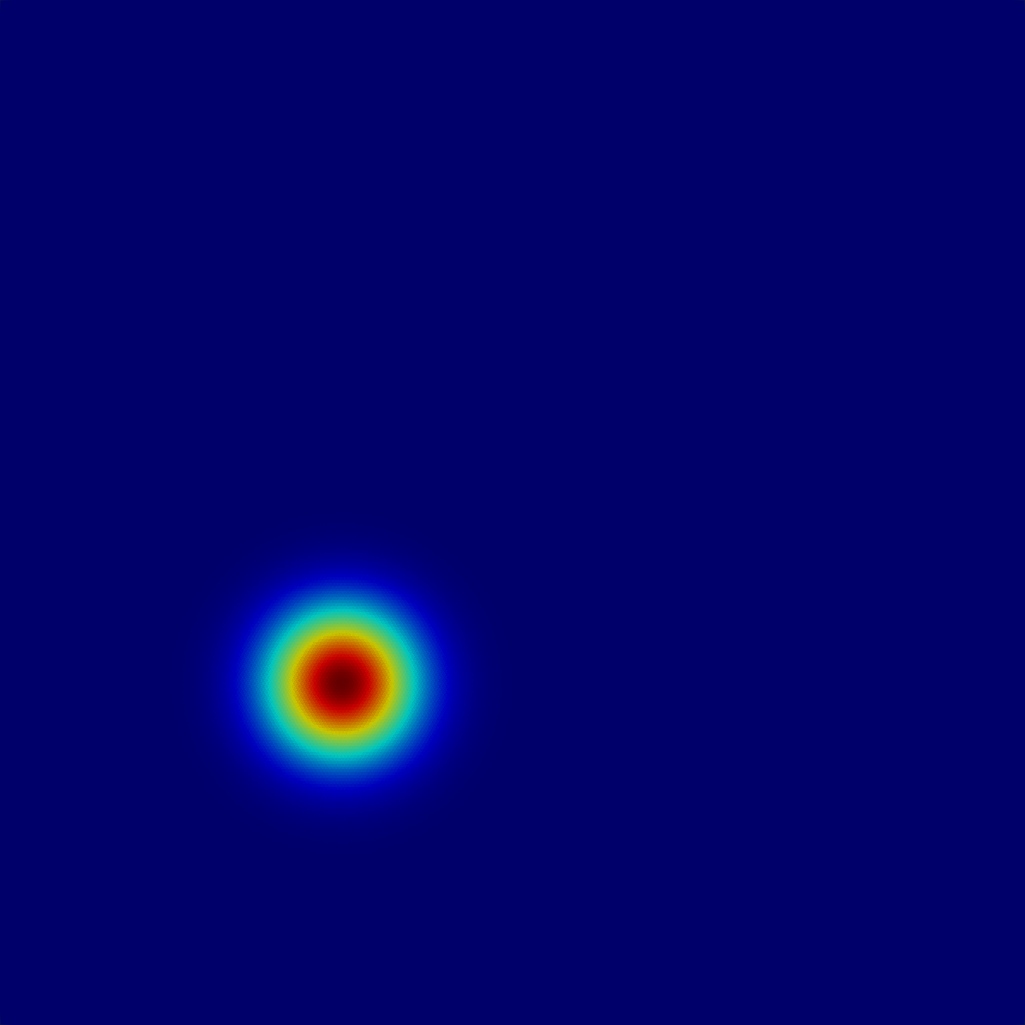
\includegraphics[width=0.4\textwidth]{advection-t0}
    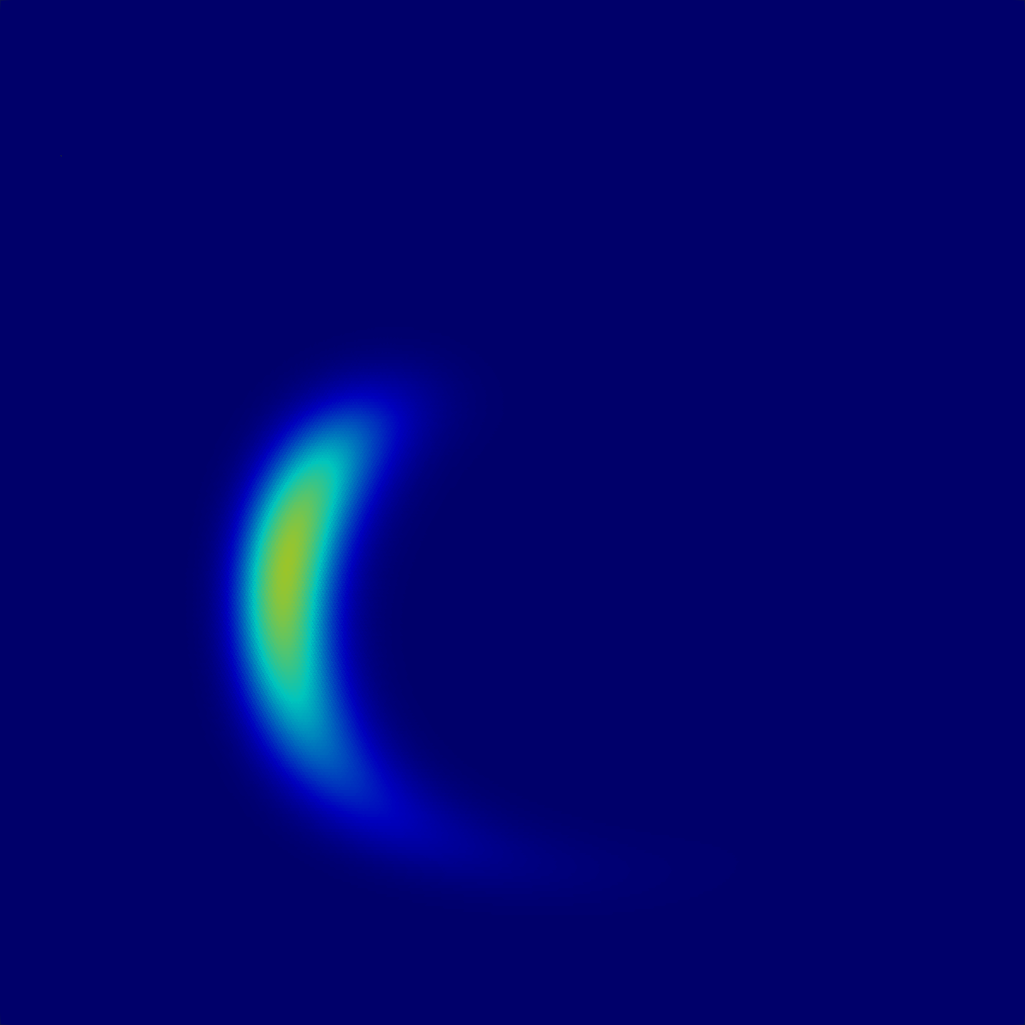
\includegraphics[width=0.4\textwidth]{advection-t5}
    \caption{Το πεδίο της βαθμωτής $U$ για χρόνο $t = 0$ (αριστερά) και χρόνο $t = 5$ (δεξιά).}
    \label{fig:advection-plot}
\end{figure}

\section{Οριακές συνθήκες}
\label{section:shockwave-bcs}

% previous example no need bcs
Το απλό παράδειγμα τις προηγούμενης ενότητας δεν απαιτεί τον ορισμό οριακών συνθηκών, καθώς το πεδίο ταχύτητας είναι παράλληλο στα όρια του υπολογιστικού χώρου, και άρα έχουμε μία de facto οριακή συνθήκη συμπαγούς τοιχώματος και σταθερής τιμής της $U$ ως 0.

% will need them for Euler
Για πιο περίπλοκα προβλήματα όμως, και ειδικά για προβλήματα ρευστομηχανικής, ο ορισμός των σωστών οριακών συνθηκών είναι πολύ σημαντικός καθώς π.χ. σε προβλήματα εσωτερικών, εξωτερικών ροών, οι οριακές συνθήκες είναι ο μοναδικός τρόπος με τον οποίο η γεωμετρία αλληλεπιδρά με το ρευστό.
Μία πρώτη προσέγγιση είναι να επεκτείνουμε τον ορισμό του προβλήματός μας, και να ζητήσουμε από τον χρήστη να ορίσει την χρονική παράγωγο για τις τιμές της λύσης πάνω στα όρια του προβλήματος.
% no time derivatives, discrete procedures
Όμως υπάρχουν πολλά είδη οριακών συνθηκών, και οι περισσότερες δεν εκφράζονται ως ένας τρόπος υπολογισμού της χρονικής παραγώγου πάνω στο όριο.
Αντίθετα, συνήθως αποτελούν διακριτούς υπολογισμούς που γίνονται στο τέλος κάθε χρονικού βήματος, και υπολογίζουν απευθείας την τιμή της λύσης πάνω στο τοίχωμα, έτσι ώστε να εξασφαλίσουν την επιθυμητή συμπεριφορά.

% use callbacks
Για την υλοποίηση τέτοιου είδους οριακών συνθηκών, το πακέτο μας χρησιμοποιεί μία χρήσιμη δυνατότητα του συστήματος επίλυσης ODE, τα λεγόμενα callbacks.
Το σύστημα callback μας παρέχει την δυνατότητα να ορίσουμε μία συνάρτηση την οποία καλεί ο επιλυτής σε διακριτές χρονικές στιγμές.
Συνήθης χρήση τέτοιων συναρτήσεων είναι η προσωμοίωση διακριτών και ασυνεχών φαινομένων, όπως είναι π.χ. η σύγκρουση δύο ελεύθερων σωμάτων.
Μπορούμε όμως να χρησιμοποιήσουμε αυτήν την δυνατότητα για να εκτελέσουμε κώδικα στο τέλος κάθε χρονικού βήματος και να εφαρμόσουμε τις οριακές συνθήκες.

Προς διευκόλυνση, το πακέτο \jlinl{Shockwave.jl}, ορίζει την βοηθητική δομή \jlinl{BoundaryCondition}, ως εξής:

{\large
\begin{jllisting}[language=julia,style=jlcodestyle]
struct BoundaryCondition{N, F}
    offset::N    # Position in memory of the first boundary element
    wallstart::N # Index of the first wall element
    wallend::N   # Index of the last wall element
    f::F         # Boundary condition function
end
\end{jllisting}
}

Ύστερα, μπορούμε να κάλεσουμε την οριακή συνθήκη ως \jlinl{bc(p, u)} για να την εφαρμόσουμε στο διάνυσμα λύσης \jlinl{u} του προβλήματος \jlinl{p}.
Τοποθετώντας αυτήν την κλήση σε ένα callback, μπορούμε να εφαρμόσουμε την οριακή συνθήκη σε κάθε βήμα.

\section{Παράδειγμα: αεροτομή σε σχήμα ρόμβου}

Ας δείξουμε τώρα την επίλυση ενός πιο ρεαλιστικού προβλήματος.
Θέλουμε να βρούμε την ροή σε σταθερή κατάσταση γύρω από μία αεροτομή σε σχήμα ρόμβου, με αριθμό Mach ελέυθερης ροής ίσο με 2.

Υποθέτουμε ότι έχουμε έτοιμο ένα μη δομημένο πλέγμα για την γεωμετρία αυτή.
Για τους σκοπούς της εργασίας, δημιουργήθηκε ένα πλέγμα 82,501 στοιχείων με το Gmsh, που φαίνεται στο σχήμα \ref{fig:mesh-diamond}.
Αν και το πλέγμα αυτό ίσως είναι λίγο μικρό, παρέχει ικανοποιητικά καλή εικόνα της ροής κοντά στην αεροτομή.

\begin{figure}[H]
    \centering
    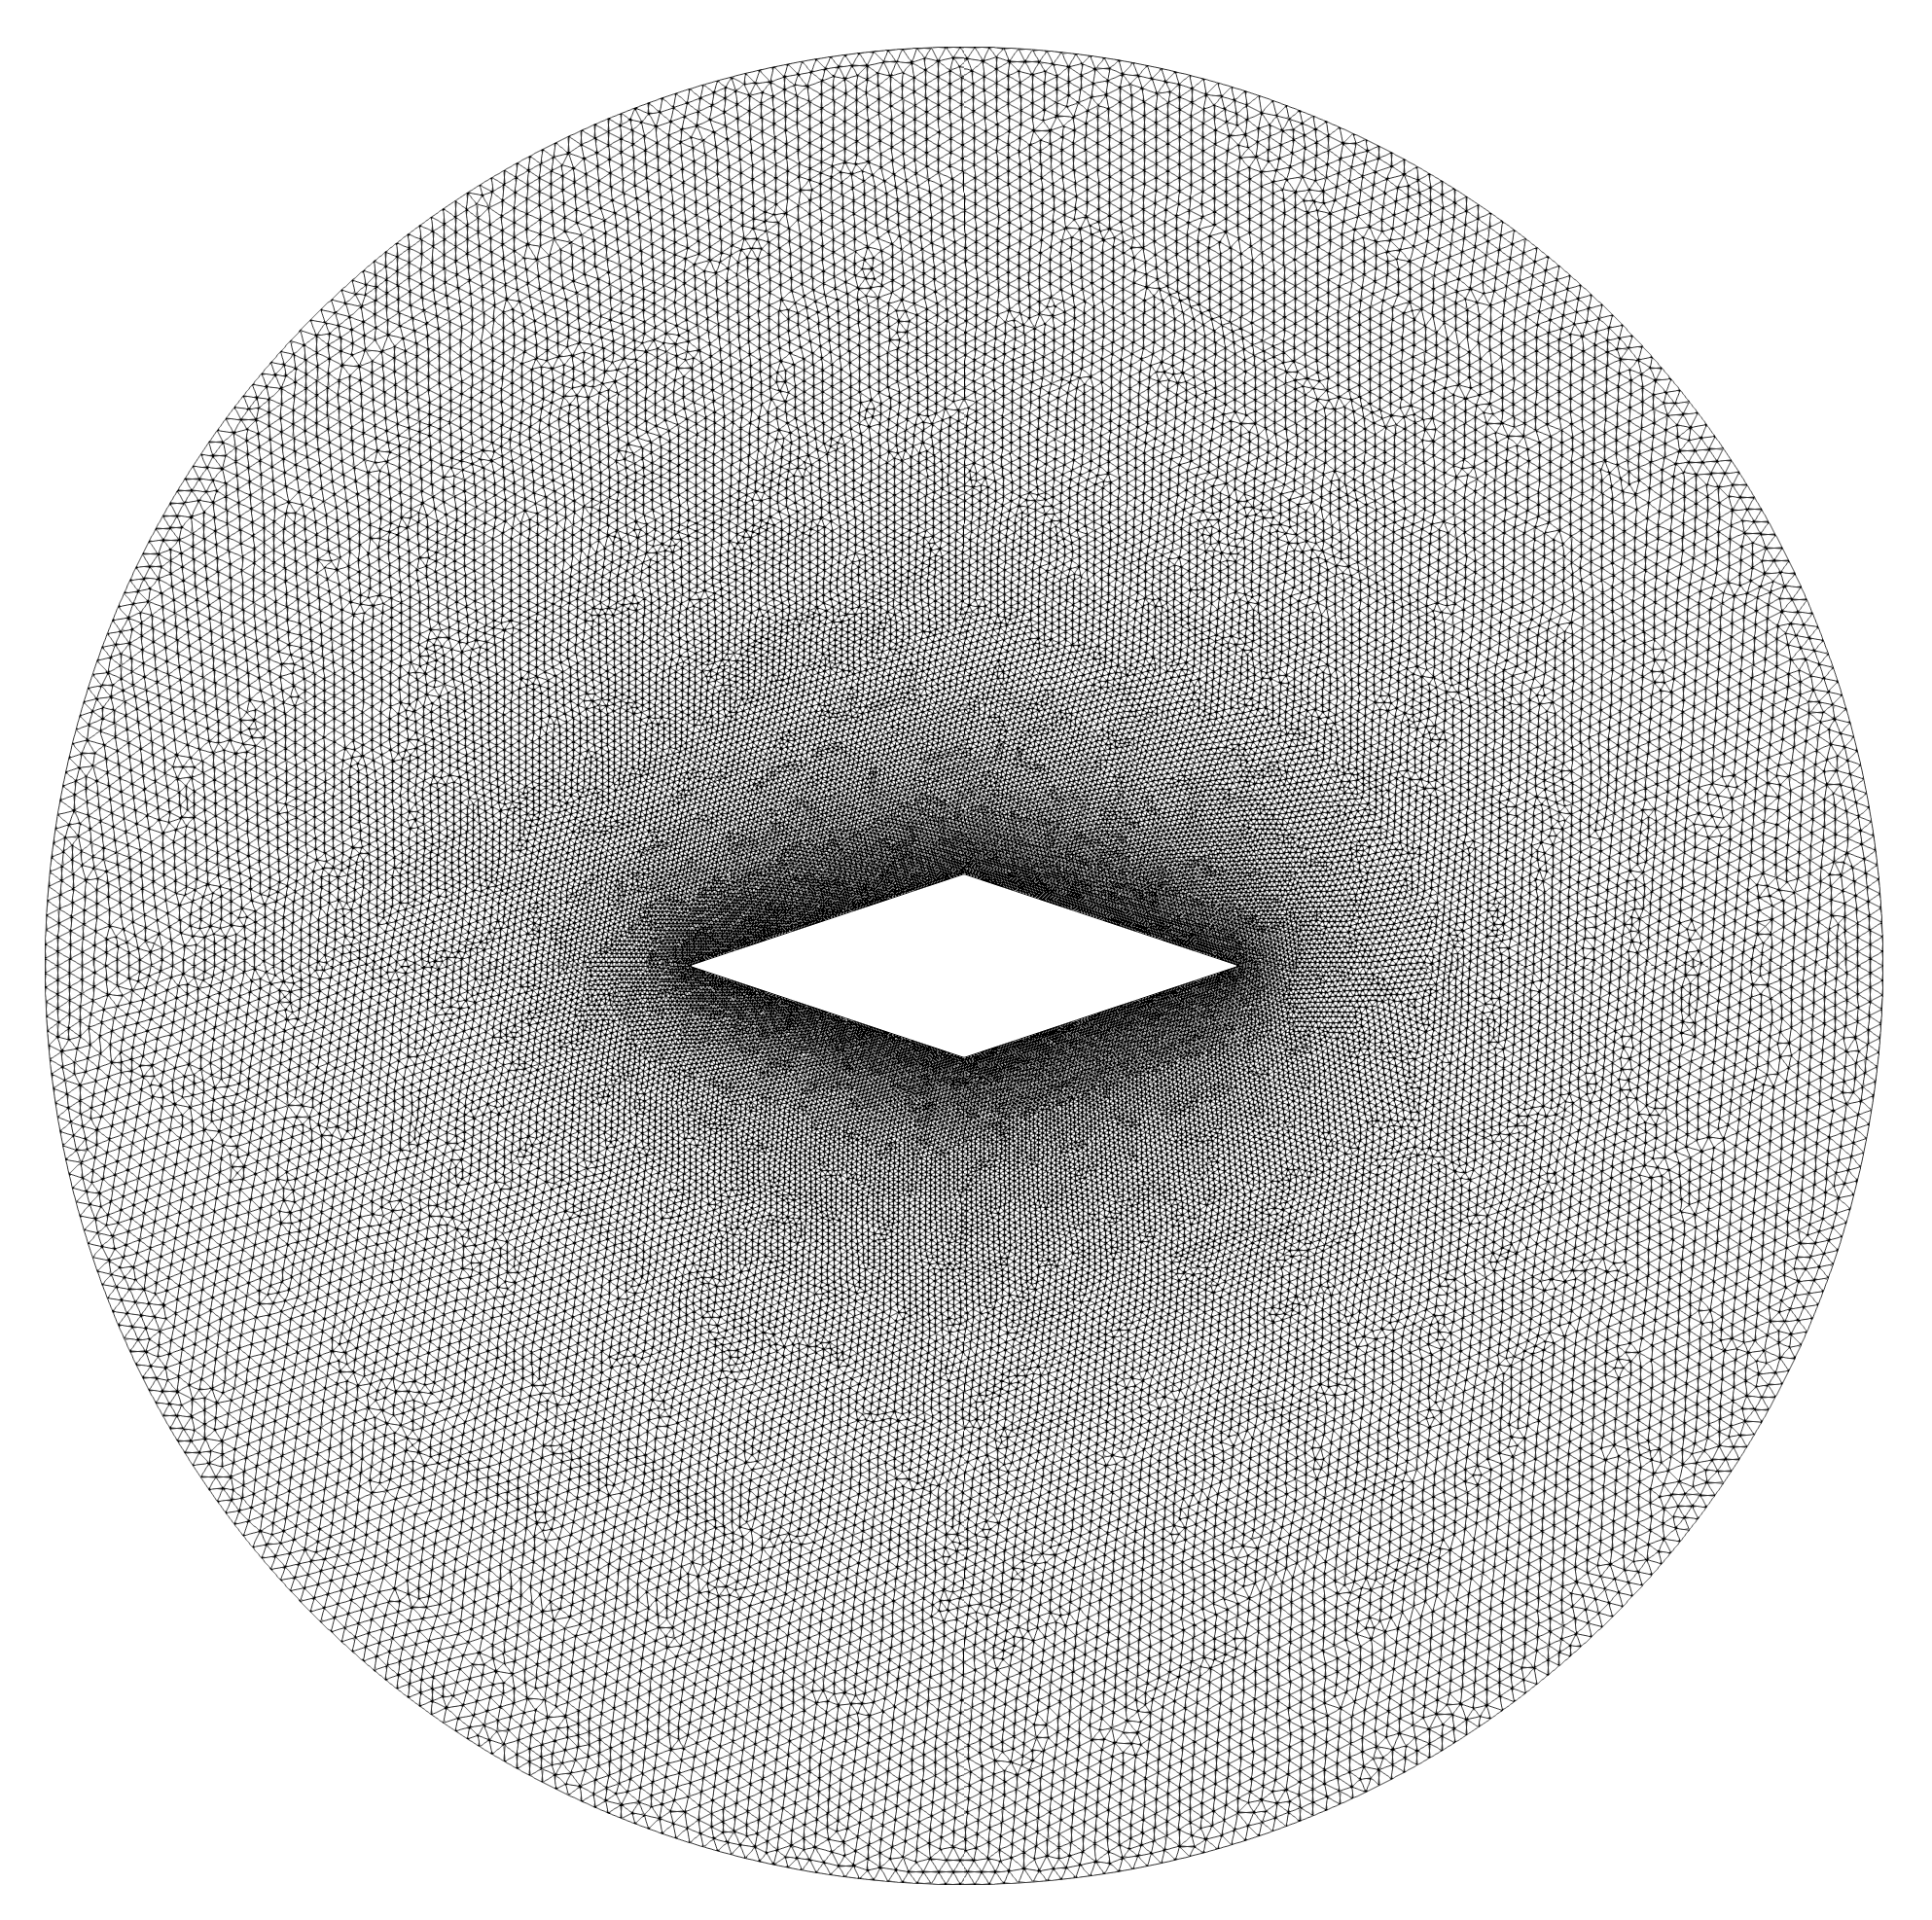
\includegraphics[width=0.8\textwidth]{diamond-mesh}
    \caption{Το πλέγμα για την επίλυση της ροής γύρω από την αεροτομή σε σχήμα ρόμβου.}
    \label{fig:mesh-diamond}
\end{figure}

Η διαδικασία της επίλυσης είναι παρόμοια με αυτήν του προβλήματος της απλής μεταφοράς της ενότητας \ref{section:square-advection}.
Για τον ορισμό της αρχικής τιμής της λύσης, υπολογίζουμε τις βαθμωτές 4 μεταβλητές των εξισώσεων Euler σε 2 διαστάσεις ως εξής:

{\large
\begin{jllisting}[language=julia,style=jlcodestyle]
farfieldu = begin
    γ = 1.4
	
    # Farfield
    p = 1e5 # N / m
    ρ = 1.161 # kg / m^2

    # Inlet conditions
	M = 2.0
	c = √(γ * p / ρ)
    v = M * c
    α = 0.0 # Angle of attack in degrees
    vx = v * cos(deg2rad(α))
    vy = v * sin(deg2rad(α))

    ρvx = vx * ρ
    ρvy = vy * ρ
    e = p / (γ - 1) + 0.5 * ρ * v^2
	
	SVector(ρ, ρvx, ρvy, e)
end
\end{jllisting}
}

Ο ορισμός του προβλήματος είναι παρόμοιος με αυτόν της προηγούμενης περίπτωσης.
Ως συνάρτηση υπολογισμού της ροής επιλέγουμε την \jlinl{Physics.Euler2D.aufs}, που παρέχουμε μαζί ως μέρος του πακέτου μας, η οποία υλοποιεί το αριθμητικό σχήμα AUFS \cite{Sun2003}.

{\large
\begin{jllisting}[language=julia,style=jlcodestyle]
fields = (:ρ, :ρvx, :ρvy, :e)
prob = AdvectionProblem(fields, Physics.Euler2D.aufs, FV1(), mesh)
\end{jllisting}
}

Για να ορίσουμε τις οριακές συνθήκες, χρησιμοποιούμε την δομή BoundaryCondition μαζί με τις έτοιμες οριακές συνθήκες που παρέχονται από το πακέτο μας, και υλοποιούν ένα τοίχωμα Euler (δηλαδή η ταχύτητα είναι παράλληλη στο όριο) και ένα μακρινό πεδίο, όπου η λύση έχει μία προκαθορισμένη τιμή εφόσον η ροή εισέρχεται στον χώρο.
Έχοντας ορίσει τα όρια Airfoil και Farfield στο πλέγμα μας, μπορούμε να τα χρησιμοποιήσουμε κατά τον ορισμό των οριακών συνθηκών ως εξής:

{\large
\begin{jllisting}[language=julia,style=jlcodestyle]
wallbc = BoundaryCondition(prob, "Airfoil", Physics.Euler2D.eulerwall)
farfieldbc = BoundaryCondition(prob, "Farfield", Physics.Euler2D.EulerFarfield(farfieldu))

function applybcs(p, u)
    wallbc(p, u)
    farfieldbc(p, u)
end

bccb = DiscreteCallback((t, u, integrator) -> true, I -> applybcs(prob, I.u), save_positions=(false, false))
\end{jllisting}
}

Μπορούμε πλέον να αρχικοποιήσουμε την λύση μας εφαρμόζοντας τις συνθήκες μακρινού πεδίου σε ολόκληρο το πλέγμα, και να προχωρήσουμε στην επίλυση του προβλήματος. Για την χρονική ολοκλήρωση, ως παράδειγμα στο συγκεκριμένο πρόβλημα μπορούμε να χρησιμοποιήσουμε έναν ολοκληρωτή Euler με χρονικό βήμα $5 \cdot 10^{-6}$ και να ολοκληρώσουμε για 50 ms, καθώς μετά από αυτό το χρονικό διάστημα η λύση είναι πρακτικά σταθερή:

{\large
\begin{jllisting}[language=julia,style=jlcodestyle]
u₀ = initfields(prob) do x, y
	farfieldu
end

odep = ODEProblem(prob, u₀, (0.0, 0.05), callback=bccb)
sol = solve(odep, Euler(); dt=dt, save_everystep=false)
\end{jllisting}
}

Αποθηκεύοντας την λύση και οπτικοποιώντας την με το ParaView, βλέπουμε το πεδίο της πυκνότητας του σχήματος \ref{fig:diamond-solution}.

\begin{figure}[H]
    \centering
    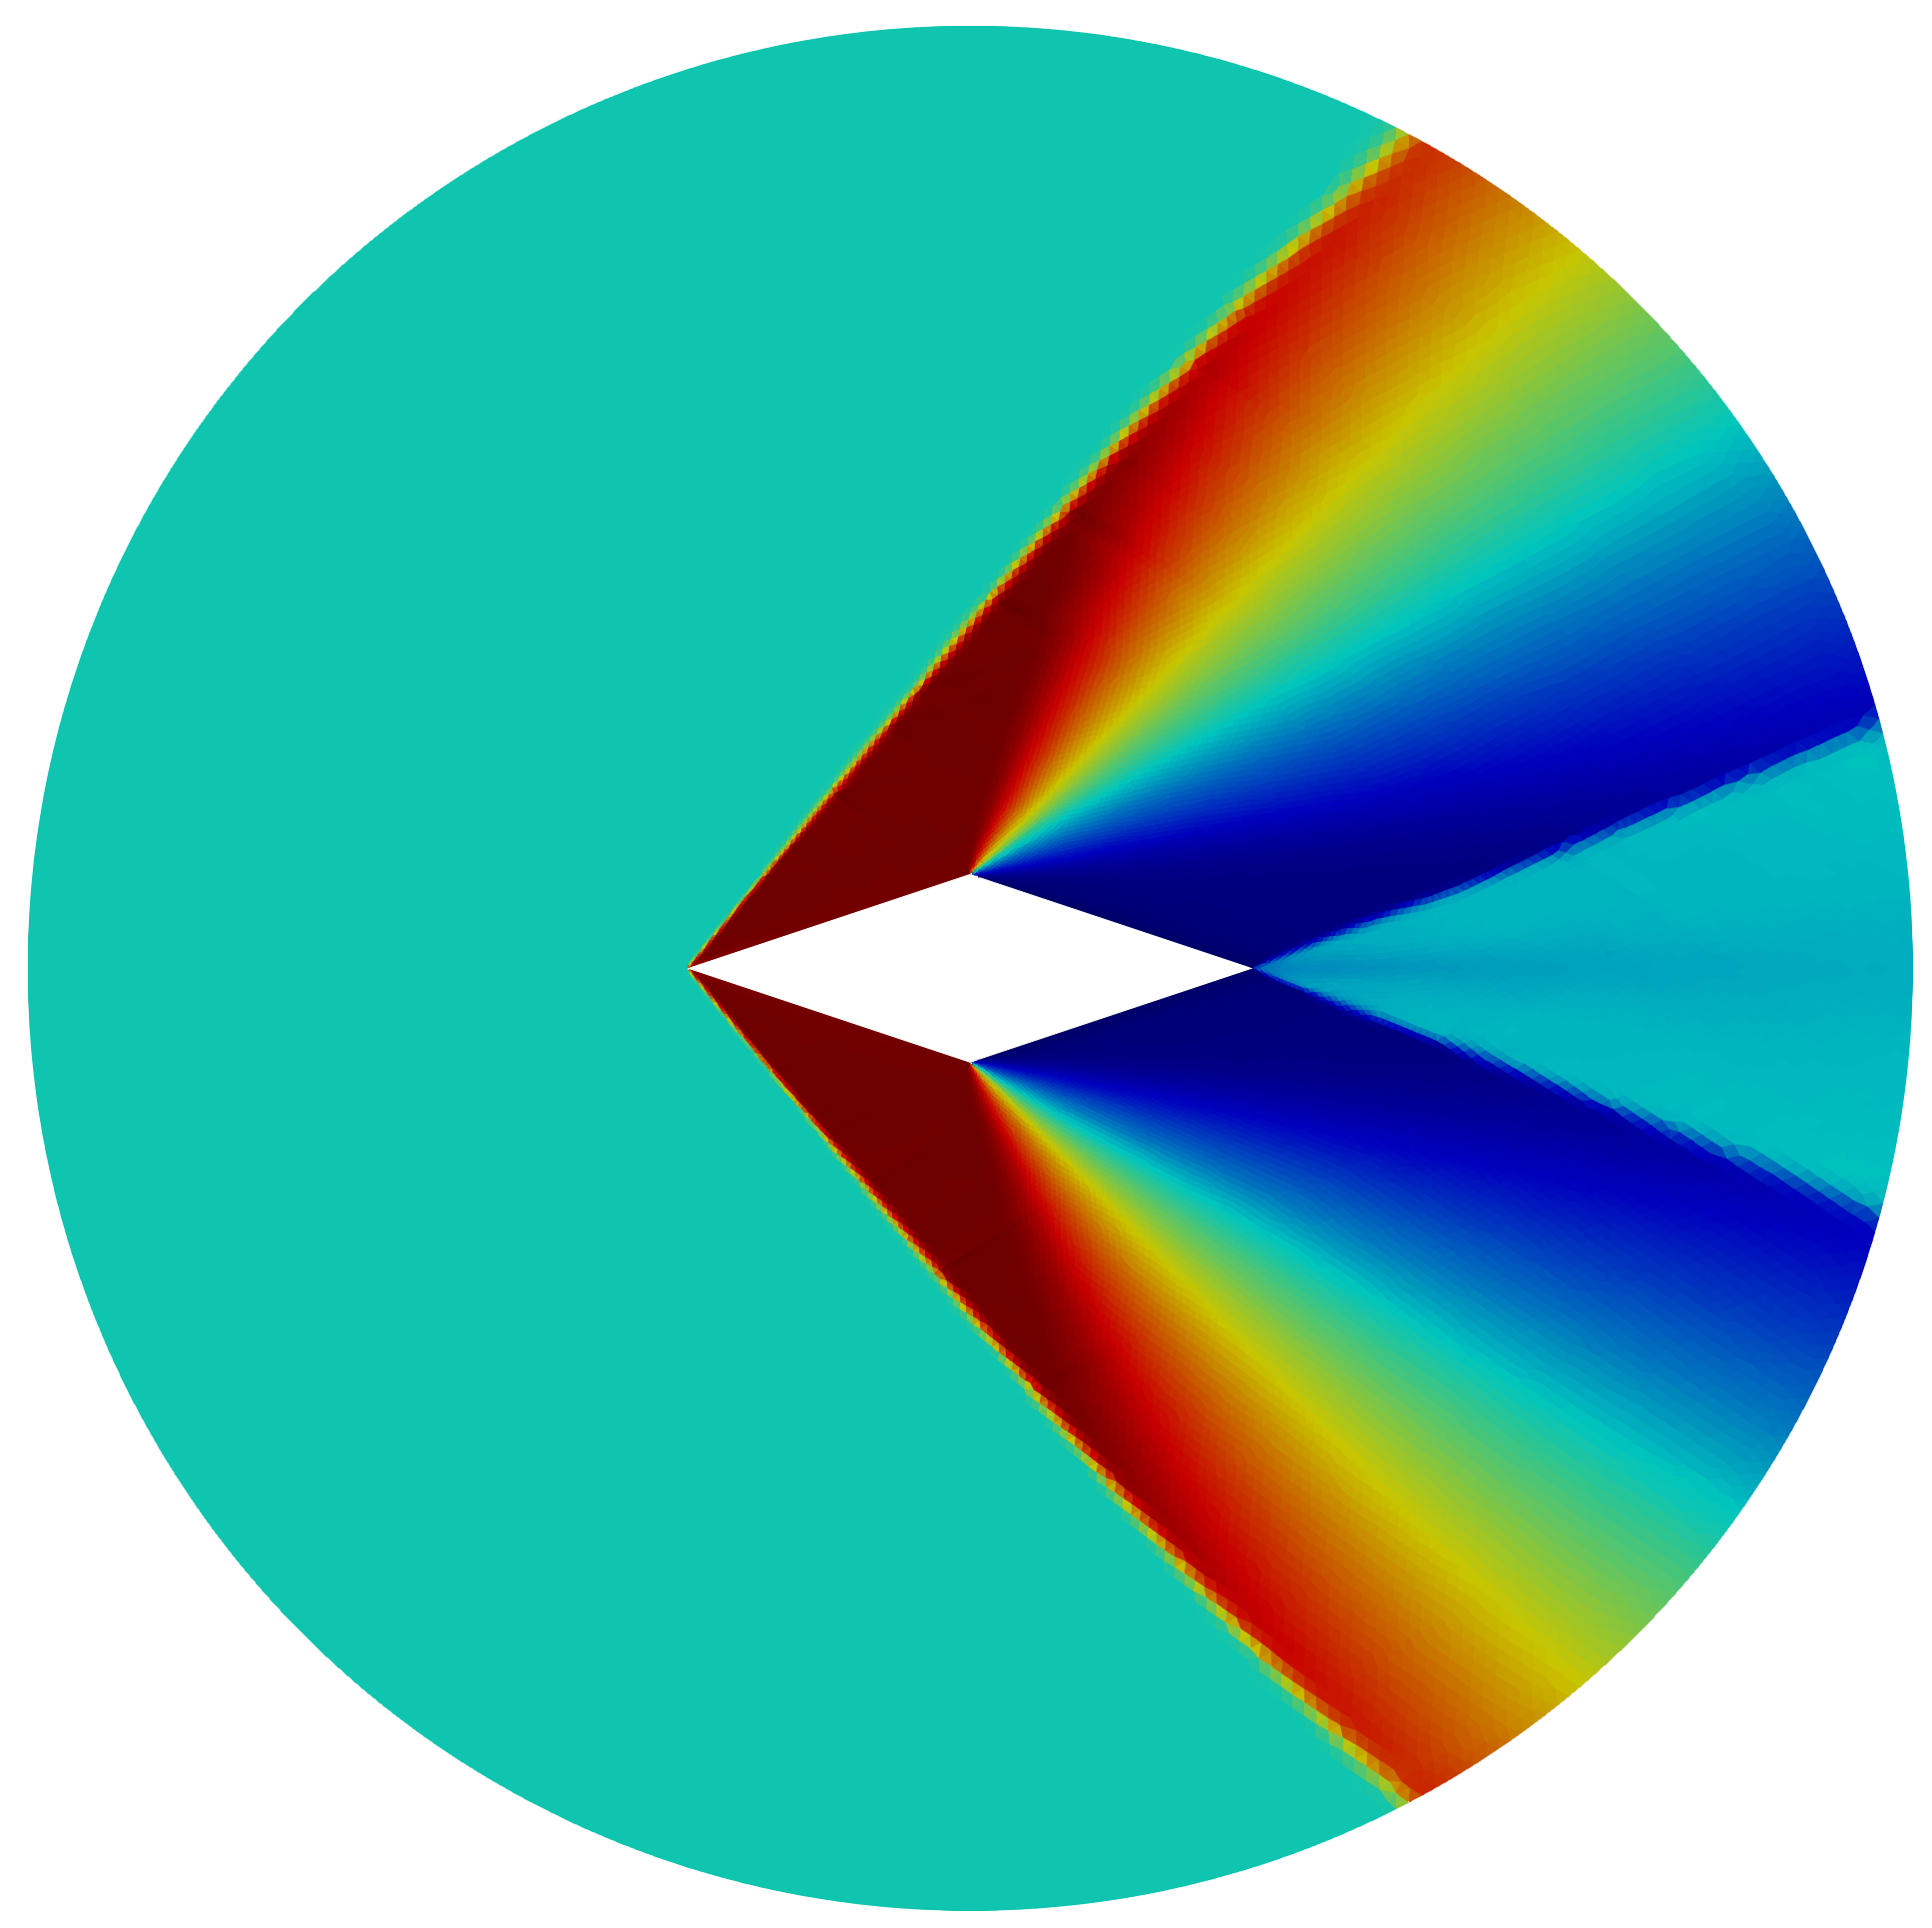
\includegraphics[width=0.8\textwidth]{diamond-solution}
    \caption{Το πεδίο της πυκνότητας στην λύση για το πρόβλημα της αεροτομής σχήματος ρόμβου.}
    \label{fig:diamond-solution}
\end{figure}

Παρατηρούμε ότι κοντά στα άκρα του χώρου της προσομοίωσης ο φυσικός ρεαλισμός του αποτελέσματος μειώνεται, κατά πάσα πιθανότητα λόγω της αλληλεπίδρασης των κρουστικών κυμάτων με την οριακή συνθήκη μακρινού πεδίου.

\section{Επιτάχυνση με CUDA}

Από την πλευρά του χρήστη, η χρήση CUDA για επιτάχυνση των υπολογισμών είναι πολύ απλή, το μόνο που χρειάζεται είναι το πρόβλημα και η αρχική λύση να μεταφερθούν στην GPU με την συνάρτηση \jlinl{cu}.
Για να μπορεί να δουλέψει αυτό, χρειάστηκε να υλοποιηθεί η συνάρτηση \jlinl{Adapt.adapt_structure}, έτσι ώστε το πακέτο \jlinl{CUDA} να μπορεί να μετατρέψει τις δομές δεδομένων μας σε δομές δεδομένων με δεδομένα στην GPU.
Πρακτικά αυτό σημαίνει ότι το μόνο που έχει να κάνει η υλοποίησή μας της συνάρτησης αυτής είναι να μετατρέψει τους εσωτερικούς πυκνούς πίνακες, όπως αυτούς που χρησιμοποιούμε για να αποθηκεύσουμε την γεωμετρία του κάθε στοιχείου, σε πίνακες \jlinl{CuArray}.

Επιπρόσθετα, χρειάστηκε να γράψουμε 2 πυρήνες CUDA, για τον υπολογισμό της συνάρτησης ροής, και την εφαρμογή των οριακών συνθηκών.
Χρησιμοποιώντας το multiple dispatch κατάλληλα, ο κώδικας είναι γραμμένος με τέτοιο τρόπο έτσι ώστε η επιλογή ανάμεσα στην υλοποίηση GPU και CPU να γίνεται αυτόματα με βάση τους τύπους δεδομένων του προβλήματος και τις αρχικής τιμής της λύσης.
Οι αλλαγές περιορίζονται σε μικρά συνδετικά κομμάτια εσωτερικά του πακέτου.
Οι συναρτήσεις υπολογισμού ροής και οι οριακές συνθήκες μπορούν να γραφούν εντελώς ανεξάρτητα της αρχιτεκτονικής εκτέλεσης τους.

\section{Εναλλακτικές προσεγγίσεις}

Η εύρεση ενός τρόπου έκφρασης αλγορίθμων επίλυσης PDE σε υψηλό επίπεδο είναι ένα πρόβλημα που έχει δεχθεί προσοχή στο παρελθόν.
Μία ενδιαφέρουσα προσέγγιση είναι αυτή της γλώσσας Liszt \cite{Liszt2011}, η οποία είναι μία γλώσσα DSL στην οποία μπορούμε να περιγράψουμε αλγορίθμους που εκτελούνται πάνω σε πλέγματα.
Η ίδια η γλώσσα δεν υλοποιεί κάποια αριθμητική μέθοδο η φυσικό μοντέλο, η συγγραφή αυτών αφήνεται για τον χρήστη.
Ο μεταγλωττιστής της Liszt δημιουργεί κώδικα C++, ο οποίος μπορεί να κάνει χρήση MPI και CUDA.

Μία εναλλακτική προσέγγιση είναι αυτή που ακολουθεί το OpenFOAM \cite{Weller1998}, το οποίο είναι η περιγραφή των διαφορικών εξισώσεων προς επίλυση με μία DSL που βασίζεται σε και μεταγλωττίζεται σε C++.
Αυτό επιτρέπει στον χρήστη να περιγράψει το φυσικό μοντέλο κατευθείαν με τις εξισώσεις που το μοντελοποιούν, αλλά παρέχει μικρότερη ευελιξία όσον αφορά την προσαρμογή του αλγορίθμου επίλυσης.

Με την έλευση της Julia το προέκυψε μία καινούργια σειρά τέτοιων προσπαθειών, καθώς η Julia καθιστά την δημιουργία DSL αρκετά εύκολη.
Ένα υπάρχον πακέτο που αναπτύσσεται γρήγορα και έχει παρόμοιους στόχους με το πακέτο της εργασίας είναι το \jlinl{Trixi.jl} \cite{Trixi2020}.
Το πακέτο αυτό επιτρέπει την επίλυση υπερβολικών συστημάτων PDE με την ασυνεχή μέθοδο Galerkin (Discontinuous Galerkin).
Δεν παρέχει δυνατότητες επιτάχυνσης με CUDA, αλλά εστιάζει σε πλέγματα που προσαρμόζονται στην λύση κατά την επίλυση (adaptive mesh refinement/AMR).
Οι εξισώσεις διατήρησης εκφράζονται παρέχοντας την συνάρτηση ροής, και το πακέτο επιτρέπει τον ορισμό βοηθητικών συναρτήσεων, για τον υπολογισμό π.χ. της ροής Godunov (Godunov flux).

